\chapter{Governing equations}

Fluid-structure interaction (FSI) combines two classical fields of mechanics, computational fluid mechanics (CFD), and computational structural mechanics (CSM). To complete FSI there is also the coupling, or interaction between these two. A separate understanding of the fluid and structure is therefore necessary to understand the full problem. This chapter presents the governing equations of the individual fluid and structure problem. Balance laws together with auxiliary kinematic, dynamic, and material relations will be described briefly.

\section{Continuum Mechanics}
In our effort to understand and describe physical phenomenon in nature, we describe our observations and theories by creating mathematical models. The mathematical models makes scientist and engineers not only able to understand physical phenomena, but also predict them.  All matter is built up by a sequence of atoms, meaning on a microscopic level, an observer will locate discontinuties and space within the material. Evaluating each atom, or \textit{material point}, is not impossible from a mathematical point of view. However, for mathematical moddeling and applications, the evaluation of each material point remains unpractical. In \textit{continuum mechanics}, first formulated by Augustin-Louis Cauchy \cite{Merodio2011}, the microscopic structure of materials are ignored,  assuming the material of interest is \textit{continuously distributed} in space, referred to as a continuum. \\

In context of this thesis we define a \textit{continuum} as a continuous body $V(t) \subset \mathbb{R}^d \ d \in (1, 2, 3)$ ,  continuously distributed throughout its own extension. The continuum is assumed to be infinitely divisible, meaning one can divide some region of the continuum a indefinitely number of times. A continuum is also assumed to be locally homogeneous, meaning if a continuum is subdivided into infinitesimal regions, they would all have the same properties such as mass density. These two properties forms the baseline for deriving conservation laws and constitute equations, which are essential for formulating mathematical models for both CFD and CSM. However, a continuum remains a mathematical idealization, and may not be a reasonable model for certain applications. In general, continuum mechanics have proven to be applicable provided that $\frac{\delta}{l} << 1$ where $\delta$ is a characteristic length scale of the material micro-structure, and $l$ is a length scale of the problem of interest \cite{Humphrey2002}.

\section{The Lagrangian and Eulerian description of motion}
In continuum mechanics, one makes use if two classical description of motion, the \textit{Lagrangian} and \textit{Eulerian} description. Both concepts are related to an observers view of motion, visually explained by the concepts of \textit{material} and \textit{spatial} points. A material points represents a particle within the material, moving with the material as it move and deform. A spatial point, refers to some reference at which the path of the material points are measured from. 

\subsubsection*{Lagrangian}
In the Lagrangian description of motion, the material and spatial points coincide, meaning the reference point of which motion is measured, follows the material as it diverts from its initial position. The initial position of all material points in a continuum extend a region, called the \textit{reference configuration} $\hat{V}$. From now on, all identities in the \textit{reference configuration} will be denoted with the notation "$\wedge$". If a continuum deviates from its reference configuration, a material point $\bat{x}(x, y, z ,t)$ may no longer be at its initial position, but moved to a new position $\mathbf{x}(x, y, z, t)$ at time $t$.  The new positions of all material points extend a new region, called the \textit{current configuration} $V(t)$. 

\begin{figure}[h!]
  \centering
    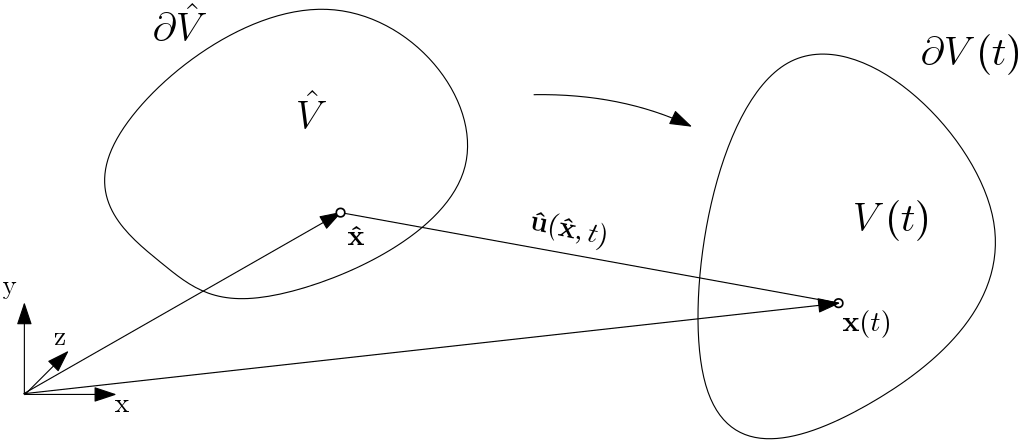
\includegraphics[scale=0.4]{./Fig/lagframe.png}
      \caption{A visual representation of the Lagrangian description of motion.}
\end{figure}

\newpage
To measure the displacement of a material point $\mathbf{x} \in V(t)$ for time $t$, from its initial point $\bat{x} \in \hat{V}$, one defines a \textit{deformation vector field} 

\begin{align}
\bat{u}(\ha{x},t) = x(\bat{x},t) - \bat{x} = \ha{T}(\bat{x}, t) 
\end{align}

Mathematically, deformation is a 1:1 mapping  $\ha{T}(\bat{x}, t)$, transforming material points from the   \textit{reference configuration} $\hat{V}$, to the  \textit{current configuration} $V(t)$. Visually, the deformation resembles the shape of continuum for some time $t$. To describe the continuums motion, one defines the \textit{velocity vector field} given by the time derivative of the deformation field,
\begin{align}
\bat{v}(\ha{x},t) = d_t x(\bat{x},t) = d_t \bat{u}(\bat{x},t) = \pder{\ha{T}(\ha{x}, t)}{t} 
\end{align}

The Lagrangian description of motion is the natural choice when tracking particles and surfaces are of main interest. Therefore, it is mainly used within structure mechanics. 

%http://www.brown.edu/Departments/Engineering/Courses/En221/Notes/Kinematics/Kinematics.htm
%Arbitrary Lagrangian-Eulerian methods J. Donea1
\subsubsection*{Eulerian}
In the Eulerian description of motion, the material and spatial points are separated. Instead of tracking material points $\hat{x}(t) \in V(t)$, the attention brought to a fixed view-point $V$. In contrary with the Lagrangian description, the \textit{current configuration} is chosen as the \textit{reference configuration}, not the initial position of all material particles. The location or velocity of any material particle is not of interest, but rather the properties of a material particle happening to be at  $\mathbf{x}(t)$ for some $t$. 

\begin{figure}[h!]
  \centering
    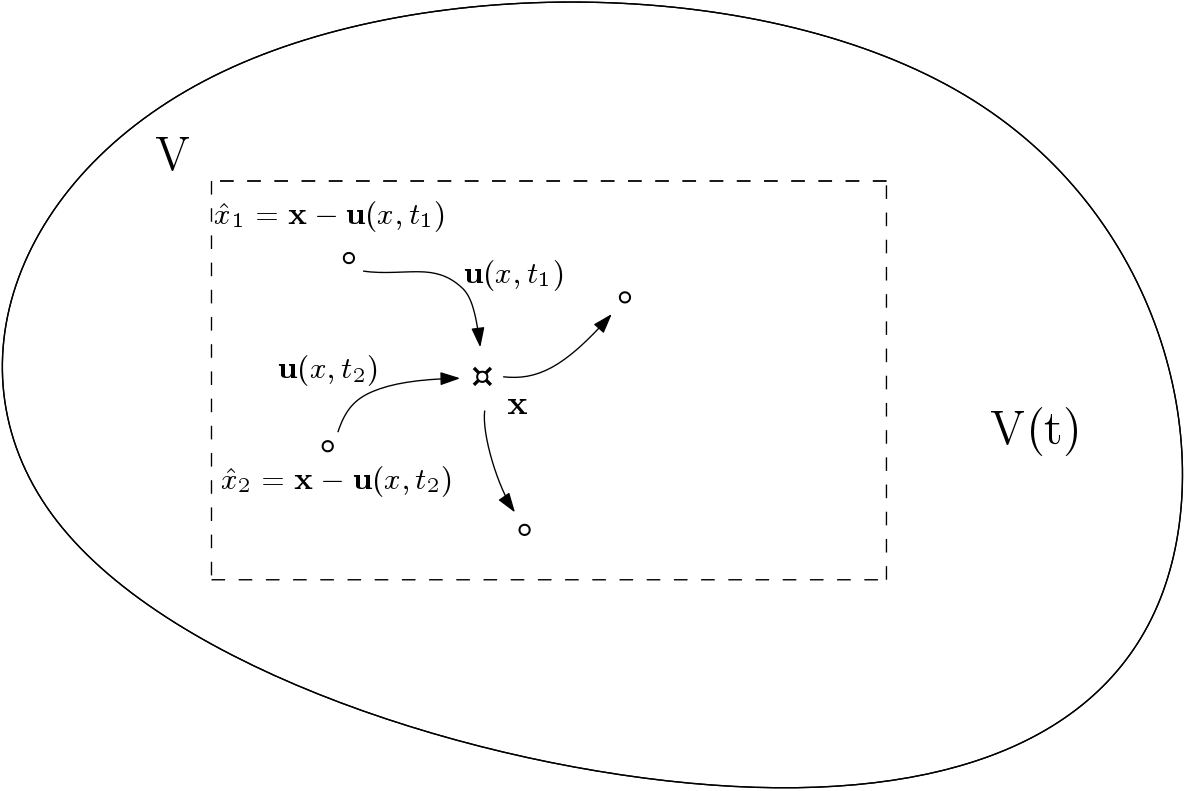
\includegraphics[scale=0.3]{./Fig/eulerian.png}
      \caption{A visual representation of the Eulerian description of motion. For a  view-point  $V$ fixed in time, a spatial coordinate $\mathbf{x}$ measures properties of a material particle $\hat{x}$ from the moving continuum  $V(t)$.}
\end{figure} 

\newpage
We can describe the particles occupying the \textit{current configuration} $V(t)$ for some time $t \geq t_0$ 
\begin{align*}
\mathbf{x} = \bat{x} + \bat{u}(\ha{x}, t)	
\end{align*}
Since our domain is fixed we can define the deformation for a particle 
occupying position $x = x(\ha{x},t)$ as
\begin{align*}
\textbf{u}(x, t) = \bat{u}(\bat{x}, t) = x - \bat{x}	\\
\end{align*}
and its velocity
\begin{align*}
\textbf{v}(\bat{x},t) = \partial_t \mathbf{u}(\bat{x},t) = \partial_t \bat{u}(\bat{x},t) = \bat{v}(\bat{x},t)
\end{align*}

The Eulerian description falls naturally for describing fluid flow, due to local kinematic properties are of higher interest rather than the shape of fluid domain. Using a Lagrangian description for fluid flow would also be tidious, due to the large number of material particles appearing for longer simulations of fluid flow. A comparison of the two previous mentioned description is shown of In Figure ~\ref{fig:lageul}.

\begin{figure}[h!]
  \centering
    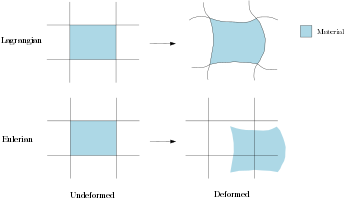
\includegraphics[scale=0.28]{./Fig/lageul.png}
      \caption{Comparison of the Lagrangian and Eulerian description of motion.}
      \label{fig:lageul}
\end{figure}


\section{The Solid problem}
\label{sec:solprob}
The solid governing equations is given by, 
\begin{equat}
\textit{Solid momentum}
\begin{align}
\rho_s \pder{\bat{v}_s}{t} = \nabla \cdot ( \hat{J} \sigma_s \bat{F}^{-T})  + \rho_s \mathbf{f}_s
\hspace{4mm} \text{in} \hspace{2mm} \hat{\Omega}_s \\
\pder{\bat{v}_s}{t} = \bat{u_s} \hspace{4mm} \text{in} \hspace{2mm}  \hat{\Omega}_s
\end{align}
\end{equat}
defined in a Lagrangian coordinate system, with respect to an initial reference configuration $\hat{\Omega}_s$. The structure configuration is given by the displacement $\bat{u}_s$, with the relation $\pder{\bat{v}}{t} = \bat{u}_s$ to the solid velocity. The density of the structure is given by $\rho_s$, and $\bat{f}_s$ express any exterior body forces acting. Finally, $\bat{F} = I + \nabla \bat{u}_s$ is the deformation gradient, and $\hat{J}$ is the determinant of $\bat{F}$ \textit{(See Appendix ~\ref{appendix:defgrad}  for further detail)}. \\

Material models express the dependency between strain tensors and stress. The validity of material models is often limited by their ability to handle deformation and strain to some extent, before it breaks down or yields nonphysical observations of the material. In this thesis, we assume a linear relation between stress and strain, where the elasticity of the material is expressed by the \textit{Poisson ratio} $\nu_s$, \textit{Young modulus} E, or Lamè coefficients  $\lambda_s$ and $\mu_s$. Their relation is given by,

\begin{align*}
&E_y = \frac{ \mu_s ( \lambda_s + 2 \mu_s) }{ ( \lambda_s + \mu_s ) } 
\hspace{5mm} \nu_s = \frac{\lambda_s}{2(\lambda_s + \mu_s)} \\
&\lambda_s = \frac{\nu E_y}{(1 + \nu_s)(1 - 2\nu_s)} \hspace{4mm} \mu_s = \frac{E_y}{2(1 + \nu_s)} 
\end{align*}


The first order \textit{Hooke´s law}, is applicable for small-scale deformations,
\begin{defn}
Let $\hat{u}$ be a differential deformation field in the \textit{reference} configuration, $I$ be the Identity matrix, and the gradient $\hat{\nabla} = (\frac{\partial}{\partial x}, \frac{\partial}{\partial y}, \frac{\partial}{\partial z}) $. \textit{Hooke's law} is then given by,
\begin{align*}
&\sigma_s = \frac{1}{\hat{J}} \bat{F}(\lambda_s(Tr(\epsilon) I + 2 \mu  \epsilon)\bat{F} \\
&\bat{S}_s = \lambda_s(Tr(\epsilon) I + 2 \mu \epsilon \\
&\epsilon = \frac{1}{2}(\hat{\nabla} \bat{u} + (\hat{\nabla} \bat{u})^T ) 
\end{align*} 
\end{defn}

Hooke's law is however limited to a small-deformation regime, and fails for larger deformations encountered in this thesis. A valid model for larger deformations is the  hyper-elastic \textit{St. \@ Vernant-Kirchhoff model}(STVK), 
extending Hooke's law into a non-linear regime.

 \begin{defn}
Let $\hat{u}$ be a differential deformation field in the \textit{reference} configuration, $I$ be the Identity matrix and the gradient $\hat{\nabla} = (\frac{\partial}{\partial x}, \frac{\partial}{\partial y}, \frac{\partial}{\partial z}) $. The \textit{St. Vernant-Kirchhoff model} is then given by the relation,
\begin{align*}
&\sigma_s = \frac{1}{\hat{J}} \bat{F}(\lambda_s(Tr(\bat{E}) I + 2 \mu \bat{E})\bat{F}^{-T} \\
&\bat{S}_s = \lambda_s(Tr(\bat{E}) I + 2 \mu \bat{E} \\
&\bat{E} = \frac{1}{2}(\bat{C} - I ) \hspace{4mm} \bat{C} = \bat{F}\bat{F}^{-T}
\end{align*} 
\textit{where $\bat{C}$ is the right Cauchy-Green strain tensor and $\bat{E}$ is the Green Lagrangian strain tensor
(See appendix B for definition)}
% (See appendix ~\ref{appendix:strainapp} for definition)}
\end{defn}
  

Though STVK can handle large deformations, it is not valid for large strain \cite{Razzaq2010}. However since the strain considered in this thesis are small, it will remain our primary choice of strain-stress relation.

In addition, initial condition and boundary condition is supplemented for the problem to be well posed. The first type of of boundary conditions are Dirichlet boundary conditions, 
\begin{align}
\mathbf{v}_s = \mathbf{v}_s^D 
\hspace{4mm} \text{on} \hspace{2mm} \Gamma_s^D \subset \partial \Omega_s  \\
\mathbf{d}_s = \mathbf{d}_s^D 
\hspace{4mm} \text{on} \hspace{2mm} \Gamma_s^D \subset \partial \Omega_s  \\
\end{align}
The second type of boundary condition are Neumann boundary conditions
\begin{align}
\sigma_s \cdot \mathbf{n} = \mathbf{g}  
\hspace{4mm} \text{on} \hspace{2mm} \Gamma_s^N \subset \partial \Omega_s 
\end{align}
 \newpage
\section{The Fluid problem}
\label{sec:fluidprob}
The fluid is assumed to be express by the in compressible Navier-Stokes equations,
\begin{equat}
\textit{Navier-Stokes equation}
\begin{align}
\rho \pder{\mathbf{v}_f}{t} + \rho \mathbf{v}_f \cdot \nabla \mathbf{v}_f &=
\nabla \cdot \sigma + \rho \mathbf{f}_f \hspace{4mm} \text{in} \hspace{2mm} \Omega_f \\
\nabla \cdot \mathbf{v}_f &= 0 \hspace{22mm} \text{in} \hspace{2mm} \Omega_f 
\end{align} 
\end{equat}
defined in an Eulerian description of motion. The fluid density as $\rho_f$ and fluid viscosity $\nu_f$  are assumed to be constant in time, and $\mathbf{f}_s$ represents any body force. 
The fluid is assumed Newtonian, where \textit{Cauchy stress sensor} follows Hooke's law
\begin{align*}
\sigma = -p_f I + \mu_f (\nabla \mathbf{v}_f + (\nabla \mathbf{v}_f)^T
\end{align*}

As for the solid problem, boundary conditions are supplemented considering  Dirichlet boundary conditions, 
\begin{align}
\mathbf{v}_f = \mathbf{v}_f^D 
\hspace{4mm} \text{on} \hspace{2mm} \Gamma_v^D \subset \partial \Omega_f \\
p_f = p_f^D 
\hspace{4mm} \text{on} \hspace{2mm} \Gamma_p^D \subset \partial \Omega_f
\end{align}
The second type of boundary condition are Neumann boundary conditions
\begin{align}
\sigma_f \cdot \mathbf{n} = \mathbf{g} 
\hspace{4mm} \text{on} \hspace{2mm} \Gamma_f^N \subset \partial \Omega_f 
\end{align}

